\documentclass[11pt,a4paper]{article}

% ---------- Encoding / Fonts ----------
\usepackage[utf8]{inputenc}
\usepackage[T1]{fontenc}

% ---------- Packages ----------
\usepackage{graphicx}
\usepackage{amsmath,amssymb}
\usepackage{siunitx}
\usepackage{booktabs}
\usepackage{tabularx}
\usepackage[hidelinks]{hyperref}
\usepackage{float}        % for [H]
\usepackage{algorithm}
\usepackage{algorithmic}  % or algpseudocode
\usepackage{subcaption}
\usepackage{tikz}
\usetikzlibrary{arrows.meta,positioning,shapes.geometric,calc}

% References
\usepackage[numbers,sort&compress]{natbib}

% Page layout
\usepackage{geometry}
\geometry{margin=2.5cm}
% ---------- Title ----------
\title{Full-Stack 4D Path Planning for U-Space:\\
Architecture and Scalability Evaluation}

\author{
Sukhbir Singh$^{1,2}$,
Enno Nagel$^{2}$,
Bianca Isabella Schuchardt$^{2}$ \\[6pt]
\small $^{1}$Technical University of Munich (TUM), Germany \\
\small $^{2}$DLR Institute of Flight Guidance, Germany
}

\date{}

\begin{document}
\maketitle
\begin{abstract}
Urban Air Mobility (UAM) requires scalable path-planning solutions to safely integrate large numbers of eVTOL vehicles into structured low-altitude airspace. U-space, the European framework for unmanned aircraft traffic management in low-altitude airspace, relies on trajectory-based planning services to support such operations. Although routing algorithms, 4D trajectory generation, and conflict detection are well established individually, few studies report end-to-end performance results of an integrated implementation. This paper presents a full-stack 4D path-planning framework for U-space corridor operations that combines A*-based global routing on a corridor graph, CFMS-based time-parameterized trajectory generation, and NDMap-based conflict detection. The system follows a microservice-oriented architecture separating a topology service providing vertiports and corridor networks, a planner service performing routing and trajectory generation, and an interface to a U-space Service Provider (USSP). Computational performance is evaluated on a representative vertiport corridor network using sequential trajectory requests, with runtime explicitly separated into routing, trajectory generation, and total processing time.
\end{abstract}

\section*{Abbreviations}

\vspace{-0.6em}
\begingroup
\footnotesize
\renewcommand{\arraystretch}{0.88}
\begin{tabularx}{\textwidth}{lXlX}
    \toprule
    Abbreviation & Meaning & Abbreviation & Meaning \\
    \midrule
    4D & Four-dimensional & A* & A-star search algorithm \\
    API & Application programming interface & CFMS & Copter Flight Management System \\
    CPU & Central processing unit & CSV & Comma-separated values \\
    DLR & German Aerospace Center & EASA & European Union Aviation Safety Agency \\
    eVTOL & Electric vertical take-off and landing & FAA & Federal Aviation Administration \\
    FATO & Final approach and take-off area & HTTP & Hypertext Transfer Protocol \\
    JSON & JavaScript Object Notation & LDP & Landing decision point \\
    LTS & Long-term support & MSL & Mean sea level \\
    NDMap & N-dimensional map & NM & Nautical mile \\
    OD & Origin--destination & OFV & Obstacle-free volume \\
    OLS & Outer limitation surface & PTS-VPT-DSN & Prototype Technical Specifications for the Design of VFR Vertiports \\
    RAM & Random-access memory & REST & Representational State Transfer \\
    RNG & Random-number generator & TBO & Trajectory-based operations \\
    TUM & Technical University of Munich & UAM & Urban Air Mobility \\
    UAS & Unmanned aircraft system & UAV & Unmanned aerial vehicle \\
    USSP & U-space Service Provider & UTC & Coordinated Universal Time \\
    UTM & UAS Traffic Management & VFR & Visual flight rules \\
    VTOL & Vertical take-off and landing & WGS-84 & World Geodetic System 1984 \\
    \bottomrule
\end{tabularx}
\endgroup


% ---------- Content ----------
\section{Introduction}
\label{sec:introduction}

Urban Air Mobility (UAM) is emerging as a promising extension of future transportation systems. To enable the safe integration of large numbers of electric vertical take-off and landing (eVTOL) aircraft into low-altitude airspace, structured traffic-management frameworks such as the European U-space~\cite{eu_commission_2017,easa2020uspace} and the U.S. UAS Traffic Management (UTM) concept~\cite{kopardekar2016utm} have been proposed. These initiatives emphasize service-oriented architectures and trajectory-based operations to support scalable and safe airspace integration~\cite{sesar_conops_2019,sesar_master_plan_2025}. It should be noted that the U-space framework itself does not prescribe corridors: U-space services are provided within designated regions or volumes, and unmanned aircraft system (UAS) operators can plan their trajectories within those volumes. Nevertheless, UAM corridors are envisioned by some operators for early UAM implementation, with U-space services provided for a larger volume covering all UAM corridors of a region, as investigated, for example, in the SESAR project EUREKA~\cite{sesar_eureka_project}. This paper therefore addresses structured corridor operations within U-space rather than treating U-space as a corridor concept.

A central requirement in such environments is computationally efficient path planning. In dense urban scenarios, trajectory requests must be processed while respecting separation requirements and structured corridor constraints. Search-based approaches such as A* have been widely investigated for UAS routing~\cite{sahawneh2016_3d_path_planning,a_star_2d3d_comparison_utm}, alongside 4D grid-based conflict management strategies~\cite{acevedo_4d_grids_u_space}. Deconfliction in multi-dimensional trajectory spaces has also been studied in trajectory-based operations frameworks~\cite{NDMap,enea_porretta_4d_tbo_comparison}, and surveys summarize the broader range of UAS path-planning methods~\cite{ahmad2023_uav_path_planning_survey}.

In operational U-space systems, path planning is not an isolated routing problem. A selected route must be converted into a time-parameterized 4D trajectory, checked against operational constraints, and integrated into a service-oriented traffic-management workflow. Monolithic implementations of these functions may limit extensibility and independent scaling. Microservice architectures offer a modular alternative by separating concerns such as topology provision, trajectory generation, deconfliction, and authorization into dedicated services~\cite{dragoni2017microservices,matlekovic2020uav}. However, quantitative evaluations of service-oriented U-space planning systems remain limited, particularly with respect to latency decomposition, computational scaling with path distance, and the evaluated behavior of integrated conflict-checking and re-planning loops.

This paper presents a service-oriented 4D path-planning architecture for structured corridor operations within U-space and evaluates both planner-stage computational scaling and conflict-enabled behavior. Two existing DLR tools are used as building blocks. The Copter Flight Management System (CFMS) is a modular experimental flight-management and 4D trajectory generation system for unmanned multicopter and other VTOL aircraft that converts a phase-structured waypoint sequence into a dense, kinematically consistent, time-parameterized trajectory~\cite{morscheck2021cfms}. NDMap is a high-performance conflict-detection library for multi-dimensional objects that indexes trajectories in a combined space--time state space and reports separation violations between them~\cite{NDMap}. The architecture separates graph-based route planning, waypoint synthesis, 4D trajectory generation, NDMap-based deconfliction, and U-space Service Provider (USSP) interaction into distinct service responsibilities. The planner stage combines A*-based routing on a vertiport corridor graph with CFMS-based trajectory generation~\cite{morscheck2021cfms}. A CesiumJS-based frontend enables interactive visualization of the generated time-dependent trajectories~\cite{cesiumjs_software}.

The evaluated planning pipeline follows four main steps. First, A* selects a shortest corridor route on the vertiport graph. Second, waypoint synthesis augments this route with departure, climb, cruise, descent, and landing structure. Third, CFMS converts the structured waypoint sequence into a dense time-parameterized 4D trajectory. Fourth, when conflict checking is enabled, NDMap checks the candidate trajectory against previously accepted trajectories and conflict intervals are fed back to the Planning Service for request-local lateral re-routing. Each planning request in this paper corresponds to a single operator request for trajectory generation and flight-plan approval for one origin--destination vertiport pair.

The contributions of this work are:
\begin{itemize}
    \item A service-oriented U-space path-planning architecture that separates topology provision, planning, trajectory generation, deconfliction, and USSP interaction responsibilities.
    \item A CFMS-compatible waypoint-synthesis pipeline that converts A*-selected corridor routes into phase-structured inputs for 4D trajectory generation.
    \item A planner-stage latency decomposition into A* path computation, waypoint synthesis, and CFMS invocation with trajectory generation.
    \item An NDMap-based conflict-checking loop with request-local lateral re-routing by graph-edge removal and A* re-planning.
    \item A sequential Hamburg vertiport corridor-network evaluation of both planner-stage computational scaling and conflict-resolution-enabled behavior.
\end{itemize}

The remainder of the paper is organized as follows. Section~\ref{sec:related} reviews related work, Section~\ref{sec:methodology} describes the system design, Section~\ref{sec:experimental_setup} outlines the evaluation setup, Section~\ref{sec:results} presents the results, Section~\ref{sec:discussion} discusses the findings and their limitations, and Section~\ref{sec:conclusion} concludes the paper.

\section{Related Work}
\label{sec:related}

\subsection{U-space and 4D Trajectory-Based Operations}

The SESAR Master Plan situates U-space within the broader transition toward trajectory-based operations (TBO) and digitally enabled air traffic management~\cite{sesar_master_plan_2025}. Comparable developments in FAA NextGen emphasize negotiated 4D trajectories to improve predictability and capacity~\cite{enea_porretta_4d_tbo_comparison}. These initiatives highlight time-constrained trajectory management and interoperable services as key enablers of scalable urban air traffic integration.

Conflict management in discretized 4D space--time representations has been demonstrated for multi-UAS operations~\cite{acevedo_4d_grids_u_space}. In parallel, U-space service architectures have been proposed that combine monitoring, traffic management, and in-flight service functions in modular system concepts~\cite{uspace_inflight_services_architecture}. These works provide important conceptual foundations for service-oriented airspace management, but comparatively few studies report computational performance measurements for deployable planning pipelines.

\subsection{UAS Path Planning and Conflict Detection}

Corridors are only one of several airspace models proposed for low-altitude urban operations. Alternative concepts include layered airspace structures, zone-based concepts, and largely unstructured free-flight airspace; the Metropolis project related these structuring options to achievable capacity under extreme traffic densities~\cite{sunil2015metropolis,schneider2014metropolis}, comparative performance assessments of different airspace management concepts for UAM have been reported more recently~\cite{abdellaoui2025_airspace_uam}, and DLR's UAM air-traffic-management research provides a broader review of these developments~\cite{schuchardt2023_atm_uam_review}. A corridor-based model is adopted in this work because it maps naturally onto a graph representation suitable for service-oriented route planning, offers predictable and procedurally simple route structures for early UAM implementation, and is envisioned by several operators for initial corridor-based operations within U-space; the trade-off is reduced routing flexibility and potentially lower capacity compared with less structured airspace concepts.

Search-based planning methods remain widely used for UAS routing in structured airspace. In corridor-based airspace models, the routing problem can naturally be represented as a graph, where nodes correspond to vertiports or route intersections and edges represent available corridor connections. Classical shortest-path methods and heuristic search algorithms such as A* are therefore suitable choices for computing lateral routes in such networks.

A* is particularly attractive in corridor networks because an admissible distance-based heuristic can guide the search toward the destination while preserving shortest-path optimality~\cite{sahawneh2016_3d_path_planning,a_star_2d3d_comparison_utm}. However, graph search alone does not produce a complete 4D flight trajectory. The selected lateral route must still be converted into a time-parameterized trajectory that respects flight-phase structure, altitude transitions, and aircraft-performance assumptions.

Conflict detection and resolution in multi-dimensional trajectory spaces have been extensively studied within trajectory-based operations frameworks~\cite{NDMap,enea_porretta_4d_tbo_comparison}. These approaches formalize separation assessment in time-dependent state spaces and provide a foundation for integrated 4D conflict management. Nevertheless, routing, trajectory generation, and deconfliction are often evaluated as separate algorithmic components rather than as parts of a service-oriented planning pipeline.

\subsection{Microservice Architectures in UAS Applications}

Microservice architectures have gained prominence in distributed software engineering due to their modularity, separation of concerns, and potential for independent scalability~\cite{dragoni2017microservices}. Applications in UAS-related domains demonstrate benefits for maintainability, simulation integration, and flexible deployment~\cite{matlekovic2020uav}.

For U-space planning systems, such an architectural style is attractive because topology provision, route planning, trajectory generation, deconfliction, and authorization can be assigned to separate service responsibilities. However, the quantitative evaluation of such integrated planning stacks remains limited. In particular, there is still a need to understand which stage of the planner pipeline dominates latency when graph-based routing is combined with 4D trajectory generation.

\medskip
\noindent
\textbf{Research Gap.}
Existing literature establishes theoretical and architectural foundations for U-space integration, UAS routing, and trajectory-based conflict management. However, few works report service-oriented latency decomposition for a deployable 4D path-planning pipeline or evaluate conflict checking and re-planning within the same service-oriented prototype. In particular, runtime breakdowns separating graph-based route search, waypoint synthesis, and kinematically feasible trajectory generation are rarely quantified. This paper addresses that gap by evaluating planner-stage computational performance and a preliminary NDMap-based lateral re-routing loop on an exemplary vertiport corridor network.

\section{Methodology}
\label{sec:methodology}

\subsection{System Architecture and Operational Flow}
\label{sec:architecture}

The proposed framework is implemented as a set of loosely coupled services designed to generate and validate 4D trajectories for structured U-space corridor operations. The main logical components are:
(i) a \emph{Topology Registry} (Webserver) providing vertiports and the corridor network,
(ii) the \texttt{acc-trajcalc} \emph{Path Planner} responsible for route computation and CFMS-based 4D trajectory generation,
(iii) the \texttt{acc-trajdeconf} \emph{Deconfliction Service} responsible for conflict detection and resolution,
and (iv) a \emph{U-space Service Provider (USSP)} responsible for flight-plan validation, authorization, and supervision. NDMap is not part of \texttt{acc-trajcalc}; NDMap-based conflict assessment is encapsulated in the separate \texttt{acc-trajdeconf} service.

\begin{figure}[!htbp]
  \centering
  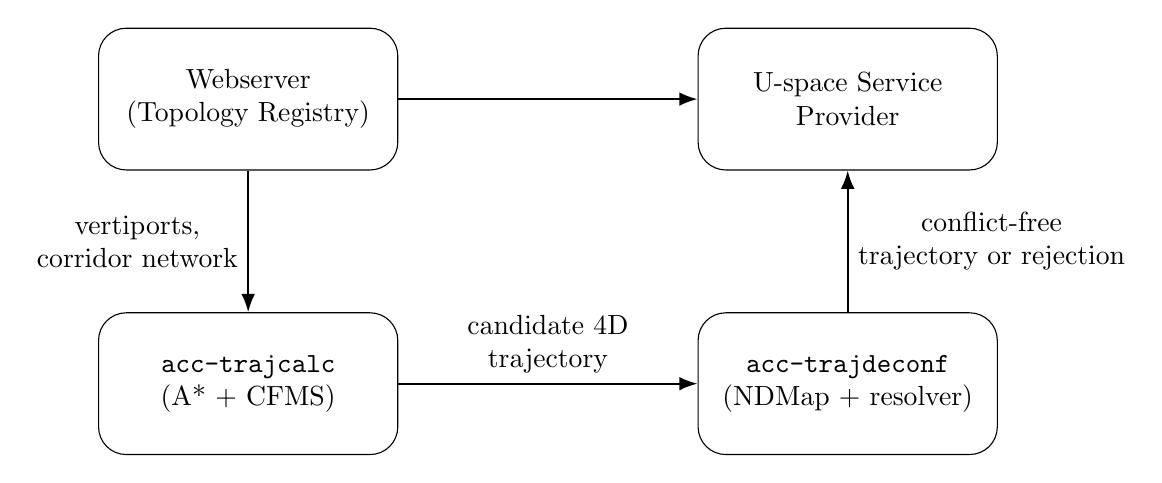
\begin{tikzpicture}[
    box/.style={
      draw,
      rounded corners=10pt,
      align=center,
      minimum width=38mm,
      minimum height=18mm
    },
    arrow/.style={-Latex, thick},
    node distance=18mm and 38mm
  ]

  % Nodes (2x2 grid)
  \node[box] (web) {Webserver\\(Topology Registry)};
  \node[box, right=of web] (ussp) {U-space Service\\Provider};

  \node[box] (planner) [below=of web] {\texttt{acc-trajcalc}\\(A* + CFMS)};
  \node[box] (deconf)  [below=of ussp] {\texttt{acc-trajdeconf}\\(NDMap + resolver)};

  % Arrows
  % Webserver -> USSP (top horizontal)
  \draw[arrow] (web.east) -- (ussp.west);

  % Webserver -> Planner (left vertical) with label
  \draw[arrow] (web.south) -- node[left, align=center] {vertiports,\\corridor network} (planner.north);

  % Planner -> Deconfliction service (bottom horizontal) with label
  \draw[arrow] (planner.east) -- node[above, align=center] {candidate 4D\\trajectory} (deconf.west);

  % Deconfliction service -> USSP (right vertical) with label
  \draw[arrow] (deconf.north) -- node[right, align=center] {conflict-free\\trajectory or rejection} (ussp.south);

  \end{tikzpicture}
  \caption{High-level service architecture separating trajectory calculation from NDMap-based deconfliction.}
  \label{fig:architecture}
\end{figure}

Fig.~\ref{fig:architecture} illustrates the high-level service interactions. The detailed internal planning workflow, including iterative conflict detection
and lateral re-routing in the deconfliction service, is depicted in Fig.~\ref{fig:planning_loop}.

\subsection{Global Route Planning on Corridor Graphs}
\label{sec:global_planning}

Global routing between vertiports is formulated as a shortest-path problem on a weighted graph \(G=(V,E)\),
where nodes \(V\) represent vertiports and edges \(E\) represent available corridor connections.
Edge weights correspond to geodesic distance between the connected endpoints (Haversine distance).
A* search is used to compute the shortest route between the selected origin and destination.
The heuristic is the straight-line geodesic distance to the destination, which is admissible and yields efficient convergence.
This heuristic is admissible because any feasible route constrained to graph edges cannot be shorter than the direct geodesic distance from the current node to the destination.
The output of this stage is an ordered list of corridor nodes:
\[
P = [v_0, v_1, \dots, v_n],
\]
which serves as the lateral (2D) reference route for subsequent trajectory generation.

% Optional (only if you want it in the paper):
% Copy your thesis A* illustration into figures/astar_graph.png and uncomment:
% \begin{figure}[!htbp]
%   \centering
%   \includegraphics[width=0.70\linewidth]{figures/astar_graph.png}
%   \caption{Illustration of A* search on the corridor graph.}
%   \label{fig:astar_graph}
% \end{figure}

\subsection{4D Trajectory Generation via CFMS}
\label{sec:trajectory_generation}

The route \(P\) is transformed into a phase-consistent four-dimensional trajectory (latitude, longitude, altitude, time) using a waypoint synthesis step and the CFMS flight-management and 4D trajectory generation system~\cite{morscheck2021cfms}.

\begin{algorithm}[htbp]
\caption{Planner pipeline for 4D trajectory generation}
\label{alg:planner_pipeline}
\begin{algorithmic}[1]
\REQUIRE Origin vertiport \(o\), destination vertiport \(d\), corridor graph \(G=(V,E)\), vertiport data, cruise altitude \(H_c\)
\ENSURE Dense trajectory \(\mathcal{T}_{\mathrm{dense}}\) and subsampled output trajectory \(\mathcal{T}_{\mathrm{out}}\)
\STATE Compute corridor route \(P\) from \(o\) to \(d\) using A* on \(G\)
\STATE Generate phase-structured waypoint sequence \(W\) from \(P\), vertiport data, and \(H_c\)
\STATE Convert \(W\) into CFMS-compatible input
\STATE Generate dense 4D trajectory \(\mathcal{T}_{\mathrm{dense}}\) using CFMS
\STATE Create subsampled output trajectory \(\mathcal{T}_{\mathrm{out}}\) with at most 200 trajectory points
\RETURN \(\mathcal{T}_{\mathrm{dense}}, \mathcal{T}_{\mathrm{out}}\)
\end{algorithmic}
\end{algorithm}

Fig.~\ref{fig:waypoint-synthesis-schematic} summarizes the waypoint-synthesis
logic used between A* routing and CFMS execution. A* provides the lateral
corridor-node sequence, while the waypoint synthesizer inserts terminal
waypoints around the departure and arrival vertiports. Intermediate A* corridor
nodes are retained as cruise-route references and marked as navigation nodes in
the waypoint list. The resulting phase-structured waypoint sequence is then
converted into CFMS input for dense 4D trajectory generation.

\begin{figure}[!htbp]
\centering
\resizebox{\linewidth}{!}{%
\begin{tikzpicture}[
    >=Latex,
    font=\small,
    route/.style={very thick, blue!70!black},
    waypoint/.style={circle, draw=black, fill=white, inner sep=1.6pt},
    aux/.style={gray!55, dashed, thin},
    leader/.style={gray!65, thin},
    labelbox/.style={font=\scriptsize, align=center, fill=white, inner sep=1.8pt},
    smalllabel/.style={font=\scriptsize, align=center, fill=white, inner sep=1.5pt},
    volume/.style={fill=blue!10, draw=blue!35, dashed, rounded corners=2pt},
    axis/.style={gray!65, thin, -Latex}
]

% ------------------------------------------------------------------
% Coordinates
% ------------------------------------------------------------------
\coordinate (origin) at (0,0);
\coordinate (depHone) at (0,1.05);
\coordinate (depHtwo) at (1.55,2.05);
\coordinate (ols) at (2.65,3.15);
\coordinate (cruiseA) at (3.55,4.20);
\coordinate (cruiseB) at (5.80,4.20);
\coordinate (cruiseC) at (8.05,4.20);
\coordinate (tod) at (9.35,4.20);
\coordinate (arrEntry) at (10.65,3.05);
\coordinate (arrHtwo) at (11.75,2.05);
\coordinate (arrHone) at (11.75,1.05);
\coordinate (ldp) at (11.75,0.55);
\coordinate (dest) at (11.75,0);

% ------------------------------------------------------------------
% Background reference lines and axes
% ------------------------------------------------------------------
\draw[axis] (-0.85,-0.35) -- (13.10,-0.35);
\draw[axis] (-0.85,-0.35) -- (-0.85,5.05);

\node[rotate=90, gray!70, font=\scriptsize] at (-1.25,2.45) {altitude / MSL};
\node[gray!70, font=\scriptsize] at (6.15,-1.15)
{progress along selected A* corridor route};

\draw[aux] (-0.55,4.20) -- (12.75,4.20);
\node[labelbox, anchor=west] at (10.15,4.45) {$H_c = 200\,\mathrm{m}$ MSL};

\draw[aux] (-0.55,2.05) -- (0.60,2.05);
\draw[aux] (11.45,2.05) -- (12.95,2.05);
\node[smalllabel, font=\small, text=black, anchor=west] at (-0.48,2.22) {$h_{2}$};

\draw[aux] (-0.55,1.05) -- (0.45,1.05);
\draw[aux] (11.45,1.05) -- (12.95,1.05);
\node[smalllabel, font=\small, text=black, anchor=west] at (-0.48,1.22) {$h_{1}$};

\draw[aux] (-0.55,0.55) -- (0.45,0.55);
\draw[aux] (11.45,0.55) -- (12.95,0.55);

% ------------------------------------------------------------------
% Terminal OFV / verticone volumes
% ------------------------------------------------------------------
\begin{scope}[on background layer]
    \path[volume]
        (-0.18,0.00) --
        (0.62,0.00) --
        (1.05,1.45) --
        (1.80,2.55) --
        (1.35,2.80) --
        (-0.18,2.80) -- cycle;

    \path[volume]
        (11.15,0.00) --
        (12.30,0.00) --
        (12.30,2.80) --
        (10.75,2.80) --
        (11.25,2.10) --
        (11.55,1.10) -- cycle;
\end{scope}

% ------------------------------------------------------------------
% Main synthesized waypoint route
% ------------------------------------------------------------------
\draw[route]
    (origin) --
    (depHone) --
    (depHtwo) --
    (ols) --
    (cruiseA) --
    (cruiseB) --
    (cruiseC) --
    (tod) --
    (arrEntry) --
    (arrHtwo) --
    (arrHone) --
    (ldp) --
    (dest);

% Waypoint markers
\foreach \p in {origin,depHone,depHtwo,ols,cruiseA,cruiseB,cruiseC,tod,arrEntry,arrHtwo,arrHone,ldp,dest}
{
    \node[waypoint] at (\p) {};
}

% ------------------------------------------------------------------
% Labels: departure side
% ------------------------------------------------------------------
\node[labelbox, anchor=north] at (0,-0.48) {origin pad\\origin};

\node[labelbox, anchor=east] at (-0.45,0.72) {vertical\\climb};
\draw[leader] (-0.10,0.72) -- ($(origin)!0.55!(depHone)$);

\node[labelbox] at (0.78,3.30) {departure OFV\\verticone};

\node[labelbox] at (2.35,1.48) {transition};
\draw[leader] (2.05,1.58) -- ($(depHone)!0.62!(depHtwo)$);

\node[labelbox] (olslabel) at (2.35,4.95) {optional\\OLS point};
\draw[leader] (olslabel.south) to[out=-90,in=120] (ols);

% ------------------------------------------------------------------
% Labels: cruise / corridor middle
% ------------------------------------------------------------------
\node[labelbox] at (5.95,5.02) {intermediate corridor nodes\\cruise references};
\draw[leader] (5.80,4.78) -- (cruiseB);
\draw[leader] (8.05,4.78) -- (cruiseC);

\node[labelbox] at (9.35,5.02) {top of\\descent};
\draw[leader] (9.35,4.78) -- (tod);

\node[
    draw=gray!55,
    rounded corners=2pt,
    fill=white,
    align=center,
    inner sep=4pt
] at (6.20,2.45)
{waypoint synthesis adds\\vertical and terminal structure\\[2pt]
 CFMS-compatible waypoint sequence\\[-1pt]
 \(\displaystyle W=[w_1,\ldots,w_m]\)};

\node[smalllabel] at (5.90,-0.58)
{\(v_1,\ldots,v_n\): A* corridor-node sequence \(P\)};

% Light gray guide dots for corridor-node sequence
\foreach \x in {1.7,3.55,5.80,8.05,9.35,10.65}
{
    \node[circle, fill=gray!45, inner sep=1.1pt] at (\x,-0.35) {};
}

% ------------------------------------------------------------------
% Labels: arrival side
% ------------------------------------------------------------------
\node[labelbox] at (11.80,3.52) {arrival OFV\\verticone};

\node[labelbox, anchor=west] at (12.55,2.38) {OFV entry};
\draw[leader] (12.35,2.30) -- (arrHtwo);

\node[labelbox, anchor=west] at (12.55,1.40) {over-pad\\waypoint};
\draw[leader] (12.35,1.18) -- (arrHone);

\node[labelbox, anchor=west] at (12.55,0.58) {LDP};
\draw[leader] (12.30,0.58) -- (ldp);

\node[labelbox, anchor=north] at (11.75,-0.48) {destination pad\\destination};

\end{tikzpicture}%
}
\caption{Schematic waypoint-synthesis procedure used to convert an A*-selected corridor route into a CFMS-compatible phase-structured waypoint sequence. The departure and arrival procedures introduce terminal waypoints at \(h_1\), \(h_2\), and the LDP, while intermediate corridor nodes define cruise-route references at the fixed cruise layer.}
\label{fig:waypoint-synthesis-schematic}
\end{figure}

\paragraph{Inputs.}
The trajectory generation stage consumes:
(i) the node sequence \(P\),
(ii) vertiport coordinates and elevations,
(iii) a fixed cruise altitude layer, and
(iv) nominal phase-dependent speeds.
In this study, the cruise layer is defined as a fixed absolute altitude of \SI{200}{m} above mean sea level (MSL). Because the altitude is defined in MSL, the height above ground may vary with terrain and pad elevation. This is a deliberate benchmark abstraction used to evaluate the computational behavior of the planning stack under controlled conditions. Accordingly, local terrain variation, obstacle constraints, and dynamic weather effects are not modeled in this stage of the evaluation, and the resulting trajectories should be interpreted as benchmark trajectories rather than operational flight plans.

\paragraph{Nominal waypoint synthesis.}
At a high level, the waypoint generator converts the lateral A* route into a
small set of phase-labeled waypoints representing departure, climb, cruise,
descent, and landing.
The lateral corridor path \(P\) is converted into a compact waypoint sequence
\(W=[w_1,\dots,w_m]\) that explicitly represents the take-off, climb, cruise,
descent, and landing phases. The first and last waypoints coincide with the
origin and destination pad locations, respectively. Between these endpoints,
\texttt{acc-trajcalc} inserts a small number of additional waypoints to shape the
vertical profile and to provide CFMS with a phase-structured route definition.

For multi-node routes, intermediate corridor nodes are retained as cruise-route
reference points. Their lateral coordinates follow the graph path, while their
altitudes are assigned according to the nominal climb profile up to the fixed
cruise layer. For direct origin--destination connections, a reduced waypoint
set is generated, including an intermediate point on the connecting geodesic to
support smooth transition between departure and arrival phases.

Each waypoint is annotated with a nominal flight phase and an associated target
speed. The phase labels distinguish terminal segments near the vertiports from
the cruise/transition segments along the corridor network. Nominal speeds are
derived from vehicle performance limits scaled by a safety factor to preserve
flyability margins.

\paragraph{Terminal procedure construction.}
The departure and arrival portions of \(W\) are generated using a simplified
vertiport terminal-procedure model. At departure, the synthesized waypoint
sequence begins at the pad elevation, continues with a vertical climb segment,
and then transitions into the outbound corridor direction. At arrival, the
sequence is constructed analogously in reverse, guiding the vehicle from the
inbound corridor segment toward the destination pad through a constrained
descent geometry.

To keep these terminal segments geometrically structured, the waypoint generator
uses a parameterized obstacle-free-volume, referred to here as a
``verticone,'' around each vertiport. Intuitively, the verticone defines a
protected three-dimensional terminal volume above and around the pad: close to
the pad the motion is mostly vertical, whereas at greater height the allowable
lateral footprint becomes wider. In this study, these geometry
parameters are taken from the EASA Prototype Technical Specifications for the
Design of VFR Vertiports (PTS-VPT-DSN), in particular the vertical take-off and
landing procedure and OFV definitions in Chapter~D, Subpart~2~\cite{easa2022_pts_vpt_dsn}. The synthesized terminal waypoints are chosen
so that departure and arrival remain inside this admissible volume.

Here, \(h_1\) denotes the lower terminal reference height, \(h_2\) the upper
terminal reference height, LDP the landing decision point, OFV the
obstacle-free volume, and OLS the outer limitation surface.
For departure, the vehicle first climbs vertically from the pad to a lower
terminal height \(h_1\). It then transitions toward a second reference height
\(h_2\) while aligning with the outbound corridor direction. If enough
horizontal distance is available, the climb can be extended farther along the
same centerline toward the outer limitation surface at up to \SI{152}{m} above
the pad, limited by the cruise altitude. For arrival, the logic is reversed:
the trajectory may first pass through a top-of-descent point on the inbound
centerline, then enters the OFV at \(h_2\), transitions to an over-pad waypoint
at \(h_1\), passes the LDP reference height, and finishes at the pad.

This procedure produces a sparse but operationally meaningful nominal waypoint
set that preserves the corridor-based lateral route while explicitly modeling
the terminal altitude transitions required before and after cruise flight.
Extended procedure-level variants such as balked landing, holding, or
energy-constrained divert trajectories exist in the implementation, but they
are outside the scope of the present evaluation.

\paragraph{CFMS execution and subsampling.}
The annotated waypoint list is converted into the CFMS input format (WGS-84 coordinates, altitudes, phase and speed fields) and passed to CFMS to produce a dense, time-parameterized trajectory \(\mathcal{T}\) satisfying the kinematic profile~\cite{morscheck2021cfms}.
To reduce payload size for downstream processing and visualization, the output representation is uniformly subsampled to a fixed maximum of 200 trajectory points while retaining the first and last samples. The trajectory generation runtimes reported in the evaluation are measured for CFMS invocation and dense trajectory generation before this subsampling step; the subsampling and visualization-export processing are accounted for separately and are not included in the planner-stage latency decomposition.

% Optional (only if you have a clear pipeline figure from thesis):
% Copy to figures/traj_pipeline.png and uncomment:
% \begin{figure}[!htbp]
%   \centering
%   \includegraphics[width=0.90\linewidth]{figures/traj_pipeline.png}
%   \caption{Trajectory generation pipeline from corridor route to time-parameterized 4D trajectory (CFMS).}
%   \label{fig:traj_pipeline}
% \end{figure}

\subsection{Deconfliction Service Using NDMap}
\label{sec:conflict_detection}

Conflict detection and resolution are performed by the separate \texttt{acc-trajdeconf} service. The service uses NDMap~\cite{NDMap}, configured over the 4D state space \((\lambda,\varphi,H,t)\) (longitude, latitude, altitude, time), to index previously accepted trajectories and identify segments of an inspected candidate trajectory that violate separation minima with respect to the active set. This keeps conflict-management state and NDMap-specific data structures outside the \texttt{acc-trajcalc} path-planning service.

\paragraph{Configuration and output.}
Separation requirements are parameterized by minimum spacing thresholds in each dimension (horizontal, vertical, and temporal).
For each detected conflict, NDMap returns one or more time intervals \([t_{\text{start}}, t_{\text{end}}]\) indicating when the candidate violates separation with any active trajectory. These intervals are used as the primary input to the resolution loop within \texttt{acc-trajdeconf}.

\begin{figure}[!htbp]
\centering
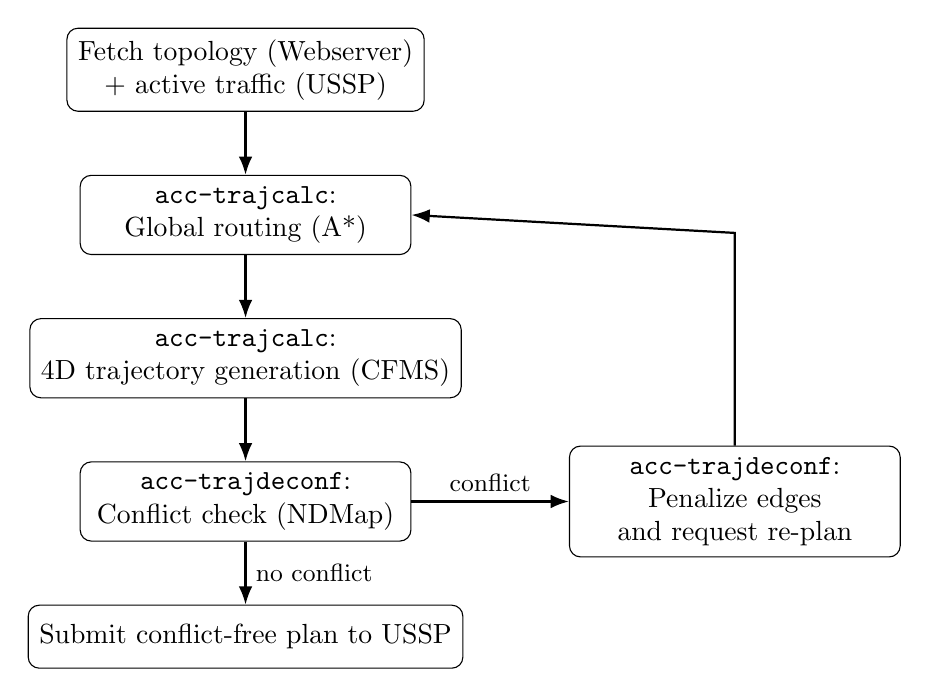
\begin{tikzpicture}[
  node distance=8mm,
  box/.style={
    draw,
    rounded corners,
    align=center,
    inner sep=4pt,
    minimum width=42mm,
    minimum height=8mm
  },
  arrow/.style={-Latex, thick}
]

\node[box] (fetch) {Fetch topology (Webserver)\\+ active traffic (USSP)};
\node[box, below=of fetch] (astar) {\texttt{acc-trajcalc}:\\Global routing (A*)};
\node[box, below=of astar] (traj) {\texttt{acc-trajcalc}:\\4D trajectory generation (CFMS)};
\node[box, below=of traj] (deconf) {\texttt{acc-trajdeconf}:\\Conflict check (NDMap)};
\node[box, below=of deconf] (submit) {Submit conflict-free plan to USSP};

\node[box, right=20mm of deconf] (penalize) {\texttt{acc-trajdeconf}:\\Penalize edges\\and request re-plan};

% Main vertical flow
\draw[arrow] (fetch) -- (astar);
\draw[arrow] (astar) -- (traj);
\draw[arrow] (traj) -- (deconf);
\draw[arrow] (deconf) -- node[right, font=\small] {no conflict} (submit);

% Conflict loop
\draw[arrow] (deconf.east) -- node[above, font=\small] {conflict} (penalize.west);

% Route return path safely below the boxes (no crossing)
\coordinate (retA) at ($(penalize.south)+(0,-6mm)$);
\coordinate (retB) at ($(astar.south)+(0,-6mm)$);

% Return path: go down, go left under all boxes, then go up to A*
\draw[arrow]
  (penalize.north) --
  ([yshift=27mm]penalize.north) --
  (astar.east);
  
\end{tikzpicture}
\caption{Operational planning loop. Candidate trajectories are generated by acc-trajcalc; conflicts are detected and resolved by acc-trajdeconf, which can trigger lateral re-routing and re-execution of A*.}
\label{fig:planning_loop}
\end{figure}

\subsection{Conflict Resolution by Lateral Re-routing}
\label{sec:conflict_resolution}

Conflict resolution is implemented in \texttt{acc-trajdeconf} using \emph{lateral re-routing} on the corridor graph. The procedure is iterative:
(1) request or receive a candidate route from \texttt{acc-trajcalc} using A*,
(2) generate the corresponding 4D trajectory through \texttt{acc-trajcalc} and perform conflict detection in \texttt{acc-trajdeconf} using NDMap,
(3) if conflicts are present, have \texttt{acc-trajdeconf} penalize corridor edges belonging to the conflicting candidate route by assigning them a very large cost (effectively removing them from consideration),
and (4) request re-execution of A* on the modified graph.
The loop terminates when NDMap reports no conflicts or when no feasible alternative route exists.

NDMap, as a trajectory-conflict management concept, can support several resolution dimensions, including changes in time, direction, and altitude~\cite{NDMap}. In the present implementation, \texttt{acc-trajdeconf} uses NDMap for conflict detection and applies resolution at the service level. The current resolution mechanism is restricted to lateral re-routing in the corridor graph; no departure-time adjustment, speed-based temporal shift, or altitude-layer change is applied.

This strategy is intentionally conservative and simple: it preserves the overall system modularity and enables scalable online admission control while illustrating how 4D deconfliction can be integrated as a dedicated microservice. More expressive resolution strategies based on temporal or vertical deconfliction are left for future work.

% Optional (use a REAL before/after figure if you have it):
% Copy to figures/conflict_before_after.png and uncomment:
% \begin{figure}[!htbp]
%   \centering
%   \includegraphics[width=0.95\linewidth]{figures/conflict_before_after.png}
%   \caption{Example of conflict handling via lateral re-routing: initial candidate trajectory conflicts with active traffic; the planner penalizes conflicting edges and produces an alternative conflict-free route.}
%   \label{fig:conflict_before_after}
% \end{figure}

\section{Experimental Setup}
\label{sec:experimental_setup}

\subsection{Scenario and Network Model}
\label{sec:scenario_setup}

All experiments were conducted on the Hamburg vertiport network considered in this work. 
Vertiports are represented as graph nodes corresponding to averaged pad coordinates, 
and air corridors are modeled as undirected edges forming a connected graph. 
Each corridor operates at a fixed absolute cruise layer of \SI{200}{m} 
above mean sea level (MSL). This fixed-altitude, obstacle-free representation is used explicitly as a benchmark abstraction for reproducible computational evaluation. Terrain elevation and obstacle variation are therefore not modeled in this study, and the corridor layer is defined in an MSL reference to ensure comparability across experiments. Edge weights are defined by the geodesic (Haversine) distance between connected vertiports.

This abstraction enables reproducible shortest-path routing while preserving 
geometrical realism at the network level.

\subsection{System Configuration}
\label{sec:system_configuration}

All experiments were executed on a workstation equipped with an 
Intel Core i7-8650U CPU @ 1.90\,GHz (4 cores, 8 threads) and 16\,GB RAM 
under a 64-bit operating system (x64 architecture).

\begin{itemize}
    \item \textbf{Operating system:} Ubuntu 24.04 LTS (Noble Numbat).
    \item \textbf{Python environment:} Project targets Python~3.14 or newer.
    \item \textbf{C++ compiler:} \texttt{g++}~13.3.0.
    \item \textbf{CFMS version:} CFMS project version~1.0.
    \item \textbf{NDMap version:} No standalone package release is declared; internal header documentation indicates version~2.00.
\end{itemize}

The Planner (Python implementation), CFMS trajectory generator (C++), and NDMap conflict detection module were executed locally on the same machine. No distributed deployment, containerization, or artificial network latency was introduced. Consequently, reported runtimes represent baseline computational performance under single-machine execution. The software follows service-oriented separation of concerns at the code and interface level; however, the evaluated implementation does not constitute a fully distributed multi-host deployment. In particular, trajectory generation and conflict detection are invoked as local native processes, and intermediate artifacts are exchanged through local filesystem paths. Therefore, while the code structure supports modular decomposition, actual horizontal scaling across multiple hosts would require additional deployment mechanisms such as shared state management, coordinated conflict-detection data access, and inter-service orchestration.

\subsection{Planner and Generator Configuration}
\label{sec:planner_configuration}

\begin{itemize}
    \item \textbf{Global planner:} A* search on the undirected corridor graph, 
    using Haversine distance both as edge cost and as admissible heuristic 
    \(f(n) = g(n) + h(n)\).
    
    \item \textbf{Cruise altitude:} Fixed absolute cruise layer of \SI{200}{m} (MSL reference), independent of local pad elevation, terrain variation, and obstacle constraints; used as a benchmark assumption rather than an operational airspace model.
    
    \item \textbf{Trajectory generation:} CFMS-based 4D synthesis with 
    phase-dependent nominal speeds derived from vehicle performance limits 
    scaled by a safety factor.
    
    \item \textbf{Sampling:} Generated trajectories were uniformly subsampled 
    to a fixed maximum number of points to reduce payload size.
\end{itemize}

\subsection{Evaluation Methodology}
\label{sec:evaluation_methodology}

To evaluate baseline computational performance, batches of trajectory requests 
were processed sequentially. For scalability analysis, 100 independent 
origin–destination vertiport pairs were randomly sampled from the corridor graph. 
Each trajectory request was fully completed before the next was initiated, 
ensuring that measured runtimes were not influenced by parallel processing effects.

In the baseline scalability experiment, conflict detection and resolution 
mechanisms were disabled to isolate the computational cost of global routing 
and trajectory generation. Runtime measurements were recorded separately for:

\begin{itemize}
    \item A* path computation,
    \item 4D trajectory generation, and
    \item total end-to-end processing time per request.
\end{itemize}

These measurements provide insight into the relative computational 
contributions of routing and trajectory synthesis within the proposed framework.

\section{Results}
\label{sec:results}

\subsection{Reference Trajectory Example}
\label{sec:reference_trajectory}

To illustrate the end-to-end planning result with one concrete and reproducible case,
we generated a reference request from vertiport `WOHL' to vertiport `KWRD' with a
specified takeoff time of 2026-03-29 06:15:00 UTC and the nominal cruise layer fixed
at \SI{200}{m} MSL. For this request, the A* planner selects the corridor sequence
\[
\texttt{WOHL} \rightarrow \texttt{HAM} \rightarrow \texttt{HOHE} \rightarrow
\texttt{HSEN} \rightarrow \texttt{HCTY} \rightarrow \texttt{TTNB} \rightarrow
\texttt{KWRD},
\]
which the waypoint synthesizer then transforms into a phase-structured trajectory with
departure climb, cruise, and arrival descent segments.

Figure~\ref{fig:reference_trajectory} shows the resulting reference trajectory both in
the horizontal plane and as an altitude-time profile. The synthesized terminal
procedure first climbs vertically from the departure pad and then transitions through
the lower terminal heights before reaching the fixed cruise layer. Along the en-route
portion, the trajectory follows the selected corridor nodes at constant cruise
altitude. Near the destination, the process is reversed through a structured descent
into the arrival pad. The resulting dense 4D trajectory spans approximately
\SI{40.6}{km} and reaches the destination at about 06:46:56 UTC, corresponding to a
flight time of roughly \SI{31.9}{min}.

\begin{figure}[htbp]
  \centering
  \begin{subfigure}[t]{0.49\linewidth}
    \centering
    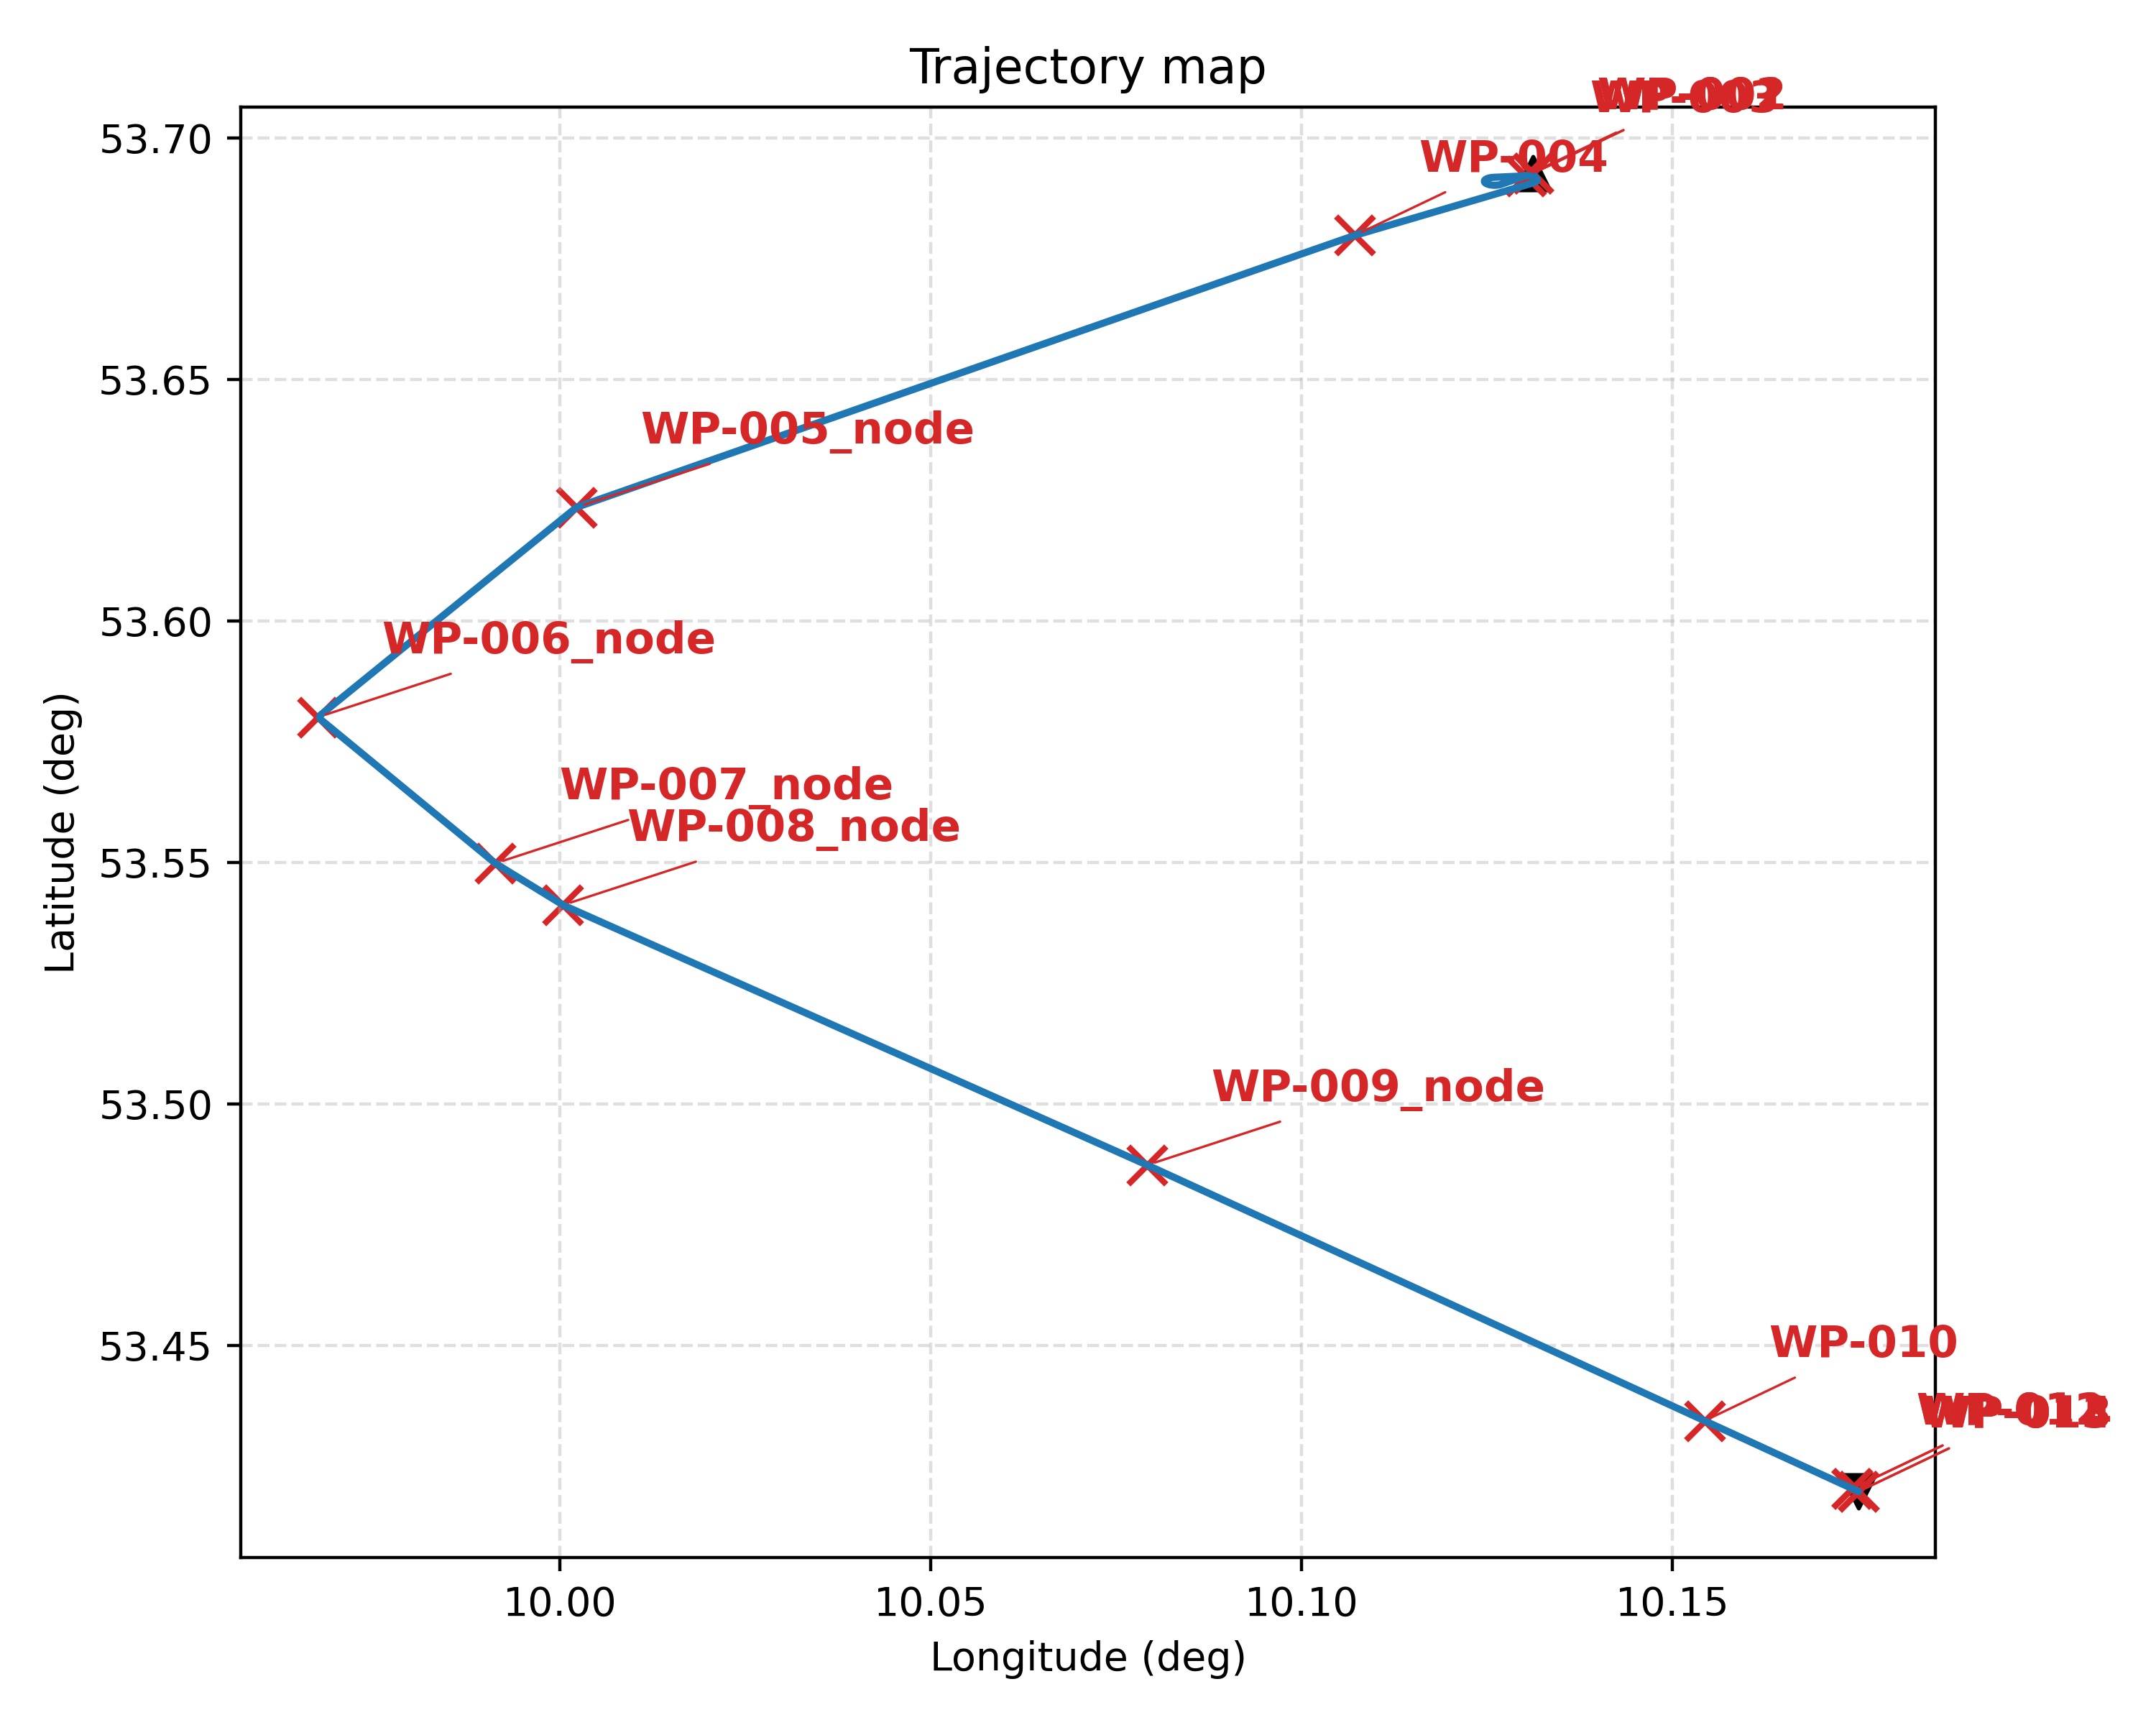
\includegraphics[width=\linewidth]{figures/reference_trajectory_map.png}
  \end{subfigure}
  \hfill
  \begin{subfigure}[t]{0.49\linewidth}
    \centering
    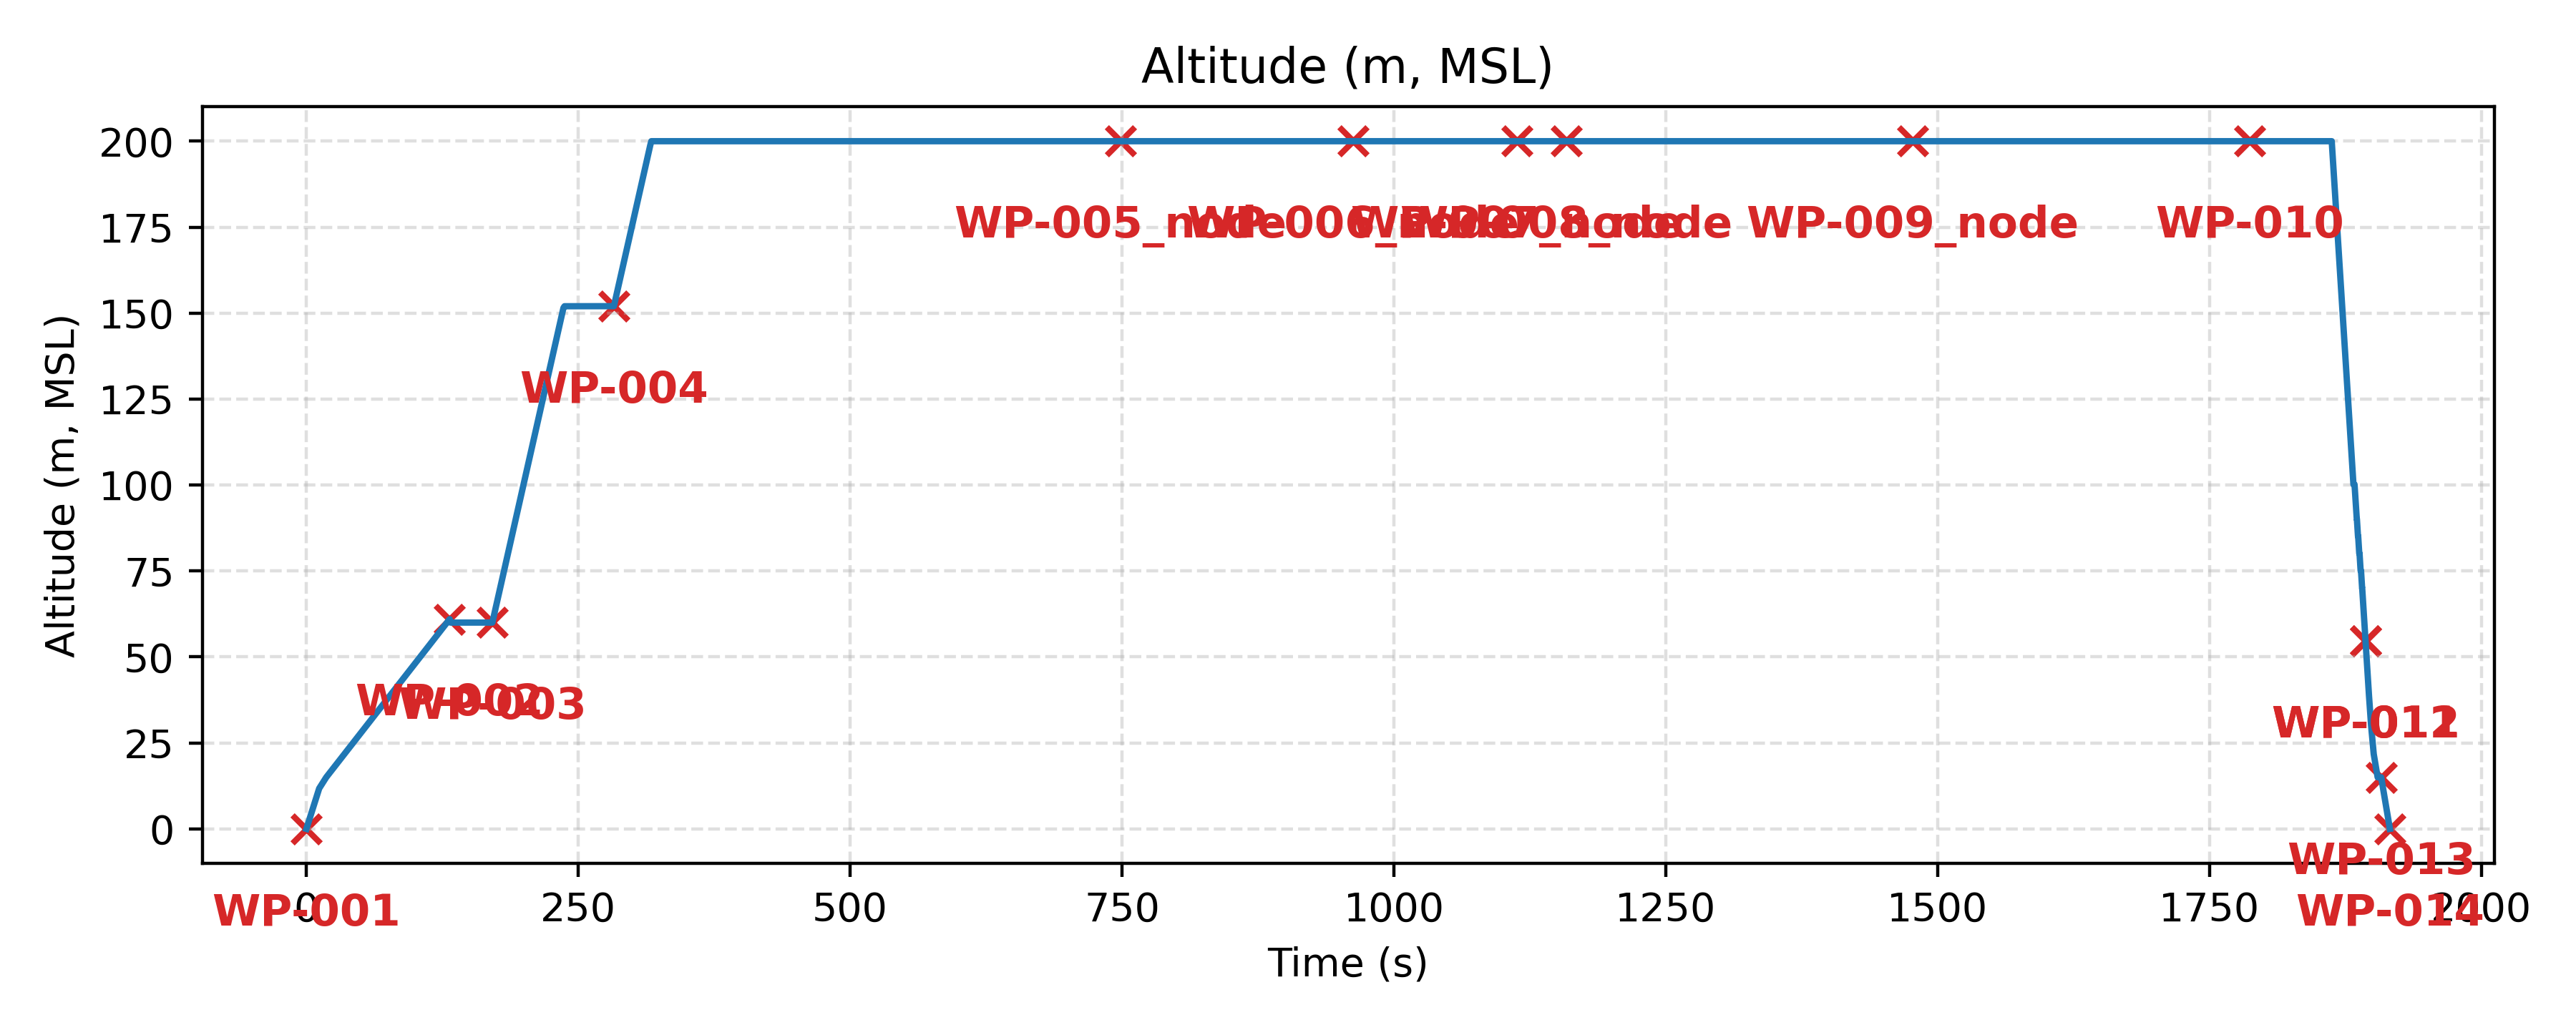
\includegraphics[width=\linewidth]{figures/reference_trajectory_altitude.png}
  \end{subfigure}
  \caption{Reference planning result for the reproducible request
  \texttt{WOHL} to \texttt{KWRD}
  at 2026-03-29 06:15:00 UTC. The left panel shows the lateral path generated from the
  A*-selected corridor sequence, while the right panel shows the corresponding
  altitude-time evolution with climb to the fixed \SI{200}{m} cruise layer and
  structured descent into the destination vertiport. Red markers indicate synthesized
  waypoints used as CFMS inputs.}
  \label{fig:reference_trajectory}
\end{figure}

\section{Discussion}
\label{sec:discussion}

The planner-stage scaling experiment shows that the evaluated service decomposition is well aligned with the computational structure of the path-planning problem. A* path search and waypoint synthesis contribute only a small fraction of the planner-stage runtime, whereas CFMS invocation and trajectory generation dominate the measured cost. For the evaluated Hamburg corridor network, graph-based routing is therefore not the main computational bottleneck; the limiting stage is converting a selected corridor route into a dense, time-parameterized 4D trajectory.

This finding is relevant for route updates and contingency planning. If a corridor edge must be removed because of a closure, geofence, or conflict-driven lateral re-routing step, the low A* runtime suggests that alternative lateral routes can be found quickly. The larger delay arises from regenerating the corresponding 4D trajectory and, when conflict checking is enabled, from repeating deconfliction against the accepted peer set.

The conflict-resolution-enabled evaluation demonstrates a preliminary NDMap and lateral re-routing loop rather than only an architectural placeholder. The prototype accepted 97 of 100 sequential requests and resolved three requests after initial conflicts by removing request-local directed graph edges and recomputing the route. The resolved cases were substantially slower because each attempt regenerated a full CFMS trajectory and repeated conflict checking. This reinforces the planner-stage finding: lateral alternatives are inexpensive to search for, but repeated 4D trajectory generation is the main cost of closed-loop re-planning.

The failed cases also define the limits of the current prototype. The retry-limit case shows that lateral-only re-routing is not sufficient for all conflicts in a single fixed cruise layer. Some encounters may require temporal shifts, speed adjustments, altitude-layer changes, or a richer search over route alternatives. The two routing/input-graph errors should not be interpreted as unresolved NDMap conflicts; they indicate implementation and integration robustness issues in the request-local re-planning loop. These failures are important for assessing the prototype, but they do not invalidate NDMap conflict detection itself.

The main optimization targets are therefore CFMS process reuse or persistent CFMS workers, adaptive trajectory sampling, route and segment caching, and clearer separation between sampling for visualization and sampling for conflict checking. More capable resolution strategies should also include temporal and vertical deconfliction, because lateral re-routing alone can exhaust available graph alternatives or produce longer trajectories without resolving the underlying encounter.

The evaluation remains limited. Requests are processed sequentially, the services run locally, the graph is small, the cruise layer is fixed at \SI{200}{m} MSL, and the scenario excludes terrain, weather, obstacle avoidance, no-fly zones, dynamic traffic demand, and concurrent service load. The results should therefore be read as a local baseline for a service-oriented prototype and not as an operational capacity assessment.

\section{Conclusion}
\label{sec:conclusion}

This paper presented a service-oriented 4D path-planning architecture for structured U-space corridor operations. The architecture separates topology provision, A*-based corridor routing, CFMS-based trajectory generation, and NDMap-based deconfliction into dedicated services. The planning pipeline first selects a corridor route, then synthesizes phase-structured waypoints, and finally generates a dense time-parameterized 4D trajectory for downstream validation and supervision.

The Hamburg vertiport corridor-network evaluation shows that A* path computation and waypoint synthesis are not the limiting stages of the evaluated planner. Both stages remain below one millisecond in the measured benchmark, while CFMS trajectory generation dominates the planner-stage runtime and largely determines the observed scaling behavior with route distance.

Future work should extend the evaluation to larger and denser corridor networks, concurrent request loads, and more operationally realistic constraints including terrain, weather, and obstacle avoidance. A further step is to evaluate the complete closed-loop interaction between trajectory generation and deconfliction, including repeated replanning triggered by detected conflicts. For the evaluated Hamburg corridor network, graph search is not the bottleneck. The main computational cost lies in CFMS-based trajectory generation, so future optimization should focus on trajectory generation, sampling, and reuse of route segments.


\section*{Acknowledgments}
% Funding/project/team acknowledgments (if needed).

\bibliographystyle{plainnat}
\bibliography{references}

\end{document}
